% SPDX-License-Identifier: Apache-2.0
%
% TxHDL, presented: the system as it is and what it does. Built by
% //docs:paper. Two columns; no history.
\documentclass[journal,9pt]{IEEEtran}

% Two columns: listings at 6pt fit 70 columns.
\newcommand{\listingsize}{\fontsize{6}{7}\selectfont}
% SPDX-License-Identifier: Apache-2.0
%
% The house preamble, shared by every document in this directory. Loaded
% after \documentclass, before \title. Keeping it in one file is what
% stops two articles drifting apart in font, listing style or figure
% style.
% Computer Modern. IEEEtran selects Times (ptm) by default, so the face has
% to be chosen explicitly.
%
% Latin Modern is the Computer Modern variety used here, and the choice is
% forced rather than aesthetic. Under T1 encoding, plain `cmr` has no Type 1
% outlines unless cm-super is installed, and it is not in the pinned
% distribution, so pdflatex falls back to EC bitmaps and every glyph in the
% PDF becomes a Type 3 font. That was measured: the first build produced a
% document with 10 Type 3 fonts and no Type 1. Latin Modern is Computer
% Modern redrawn with a full T1 repertoire and real .pfb outlines, so the
% same design comes out scalable.
\usepackage[T1]{fontenc}
\usepackage[utf8]{inputenc}
\usepackage{lmodern}
% microtype is not in the pinned TeX distribution. emergencystretch alone
% keeps the two-column measure from producing overfull lines.
\setlength{\emergencystretch}{3em}

\usepackage{amsmath}
\usepackage{amssymb}
\usepackage{amsthm}
\usepackage{booktabs}
\usepackage{array}
% enumitem is not in the pinned TeX distribution; the list spacing below
% does what \setlist would have done.
\usepackage{float}
\usepackage{xcolor}
\usepackage{listings}
\usepackage{tikz}
\usetikzlibrary{arrows.meta,positioning,fit,backgrounds,calc}
\usepackage[hidelinks,bookmarks=true]{hyperref}

% Numbered, definition-style box for a rule the reader is meant to apply.
\theoremstyle{definition}
\newtheorem{rulebox}{Rule}
\newtheorem{example}{Example}

% Unnumbered asides.
\theoremstyle{remark}
\newtheorem*{tip}{Tip}
\newtheorem*{pitfall}{Pitfall}

% Tighter lists, in place of enumitem's \setlist.
\setlength{\topsep}{2pt}
\setlength{\itemsep}{1pt}
\setlength{\parsep}{0pt}

\newcommand{\code}[1]{\texttt{#1}}
\newcommand{\term}[1]{\emph{#1}}

% Syntax highlighting. Four roles, distinguishable in colour and still
% distinguishable in greyscale, because an IEEE article gets printed: the
% keyword is the only bold role, the comment is the only italic one, and the
% two remaining roles differ in lightness as well as in hue.
\definecolor{kwblue}{RGB}{20,60,150}
\definecolor{cmtgreen}{RGB}{90,120,90}
\definecolor{strred}{RGB}{150,50,40}
\definecolor{numgray}{gray}{0.45}
\definecolor{framegray}{gray}{0.70}
\definecolor{bgshade}{gray}{0.97}
% A darker fill for figure cells. The listing background has to stay very
% light to keep code readable; a figure cell has to be clearly shaded or the
% distinction it draws is invisible in print.
\definecolor{cellshade}{gray}{0.90}

% The listing size is the document's choice, because it depends on the
% column: a two-column article sets `\listingsize` to 6pt and keeps its
% listings within 70 columns, a one-column document keeps the body size
% and includes source files at 80. Lines are never broken; a line that does not fit
% overflows the frame, which is visible, rather than wrapping, which is
% not.
\providecommand{\listingsize}{\scriptsize}

% `'` is deliberately not a string delimiter: the language uses it for loop
% labels, as Rust does, so treating it as a quote would swallow the rest of
% the line.
\lstdefinestyle{txhdl}{
  basicstyle=\ttfamily\listingsize,
  keywordstyle=\bfseries\color{kwblue},
  commentstyle=\itshape\color{cmtgreen},
  stringstyle=\color{strred},
  numberstyle=\tiny\color{numgray},
  morekeywords={mod,use,pub,const,type,struct,enum,trait,impl,fn,async,let,mut,
    match,if,else,loop,while,for,in,break,continue,return,as,await,
    module,bus,channel,transaction,protocol,pipeline,flow,seq,config,
    port,stage,pipe,instance,connect,bind,tag,domain,blackbox,foreign,
    property,role,signal,handler,true,false,
    sequence,interface,modport,implements,package,import,var,wire,func,proc,
    case,default,next,fork,branch,join,state,fsm},
  morecomment=[l]{//},
  morestring=[b]",
  showstringspaces=false,
  columns=fullflexible,
  keepspaces=true,
  breaklines=false,
  % Framed, so a listing is bounded rather than floating in the column.
  frame=single,
  rulecolor=\color{framegray},
  framesep=3pt,
  backgroundcolor=\color{bgshade},
  xleftmargin=3pt,
  xrightmargin=3pt,
  aboveskip=6pt,
  belowskip=6pt,
  % Every listing is numbered and captioned, so it can be referred to by
  % number. `caption` without `float` numbers the listing and leaves it
  % where it was written, which is what a listing in running prose needs.
  captionpos=b,
  abovecaptionskip=2pt,
  belowcaptionskip=6pt,
}

% Figures drawn as text. Framed the same way, and with the highlighting
% switched off, because a box-and-arrow diagram is not code and half its
% words turning blue reads as an accident. Setting a style adds keys rather
% than clearing the ones already set, so the three roles are neutralised by
% hand rather than by leaving them out.
\lstdefinestyle{ascii}{
  basicstyle=\ttfamily\listingsize,
  keywordstyle=\ttfamily,
  commentstyle=\ttfamily,
  stringstyle=\ttfamily,
  columns=fullflexible,
  keepspaces=true,
  frame=single,
  rulecolor=\color{framegray},
  framesep=3pt,
  backgroundcolor=\color{bgshade},
  xleftmargin=3pt,
  xrightmargin=3pt,
  aboveskip=6pt,
  belowskip=6pt,
}
\lstset{style=txhdl}

% House TikZ styles. `shorten` lives on the arrow styles rather than on each
% arrow, so every arrow in the document gets the gap, including ones added
% later. TikZ clips a path at a node's border, so without it an arrowhead
% butts against the box with no gap at all. Keep `node distance` well above
% twice the shorten, or the arrow shrinks to nothing.
\tikzset{
  box/.style={draw,rounded corners=2pt,align=center,inner sep=4pt,
              font=\footnotesize},
  boxf/.style={box,fill=bgshade},
  lbl/.style={font=\scriptsize\itshape,align=center},
  fl/.style={-{Stealth[length=4pt]},shorten >=2.5pt,shorten <=2.5pt},
  fld/.style={fl,dashed},
}



\InputIfFileExists{buildstamp.tex}{}{}
\providecommand{\buildstamp}{Draft build (outside the Bazel flow).}

\definecolor{tint}{RGB}{232,238,250}
\tikzset{
  box/.style={draw, rounded corners=2pt, minimum height=6mm, inner sep=3pt, align=center, font=\small},
  art/.style={draw, fill=tint, rounded corners=2pt, minimum height=6mm, inner sep=3pt, align=center, font=\small},
  chk/.style={draw, fill=green!12, rounded corners=2pt, minimum height=6mm, inner sep=3pt, align=center, font=\small},
  flow/.style={-{Stealth[length=2mm]}, thick},
  lbl/.style={font=\scriptsize, fill=white, inner sep=1pt},
}

\title{TxHDL: A Hardware Description Language\\That Is a Rust Library}

\author{Filip Filmar and Dragiša Janković%
\thanks{Both authors are independent. Filip Filmar is the
corresponding author, at f@hdlfactory.com; Dragiša Janković is
reached at linkedin.com/in/dragisa-jankovic.}%
\thanks{This paper presents TxHDL as it stands: the language, its
runtime, the traces and netlists it produces, the checks that hold
them together, and the Vreteno RV32IM core built with it. Every
listing is included from the project repository \code{HDL/txhdl} at
build time, every waveform is drawn from a trace the build produced,
and every number is from a run the build made. The companion
documents~\cite{cover} hold the rest.}%
\thanks{The authors used a large language model, Claude, as an
assistant in exploring the concepts and in writing and constructing
the documents and the programs; every commit of the repository says
so and carries the prompts that led to it, verbatim.}%
\thanks{\buildstamp}}

\markboth{TxHDL}{Filmar and Janković: TxHDL}

\begin{document}
\maketitle

\begin{abstract}
TxHDL is a hardware description language with no grammar of its own.
A design is a Rust program: a unit is a struct, its state is a field,
its behaviour is an \code{async fn} that waits for clock edges, and a
value that lives across a wait is a register the source never named.
The language is a library and a few macros; the parser, the type
checker, the module system and the tooling are Rust's. The same
source runs as a cycle-accurate simulation, writes a waveform, and
lowers to a netlist in Verilog and VHDL, and the build simulates that
netlist under nvc and Verilator against the trace the simulation
wrote, so a design that passes is right in three forms at once. The
largest design so far is Vreteno, a three-stage RV32IM core with
machine-mode traps, an interrupt line and a bus with its data
memory, a timer and a serial port on it: written in the subset the
lowering reads, checked
in lockstep against a reference model, checked as a netlist against
its own trace, synthesized, placed and routed on an Artix-7 at
100~MHz in 2041 LUTs, its data memory a device in block RAM, and run
on the board, where it said on its serial port what the simulation
had said. The language is proven on hardware. This paper presents
the system and its results.
\end{abstract}

\begin{IEEEkeywords}
Hardware description languages, embedded domain-specific languages,
Rust, RISC-V, high-level synthesis.
\end{IEEEkeywords}

\section{Introduction}
\label{sec:p-intro}

\IEEEPARstart{A}{} hardware description language usually arrives with
a parser, a type checker, a module system and an editor of its own,
each written once more. TxHDL does not. It starts from a
specification of a language shaped like Rust and deletes every
construct Rust already provides: structs, generics, traits, modules,
functions, \code{async} and \code{await}. What remains is the part
that means hardware, and it fits in a library of five modules and a
handful of macros. A design is an ordinary Rust crate, compiled by
\code{rustc}, and the type checker finds two drivers on a wire, a
clock-domain crossing without a synchroniser, and a cycle count in a
combinational body, as type errors.

That library is also a runtime. A design runs as a simulation with a
stated model of time, one process per unit, and writes a waveform in
FST or VCD. It is also the input of a lowering: an attribute on a
unit reads its \code{run} loop and emits Verilog and VHDL, and the
build simulates the netlist against the trace the Rust simulation
wrote, under two simulators, so the three forms of a design are held
to one behaviour. Fig.~\ref{fig:p-system} shows the whole.

\begin{figure}[htbp]
\centering
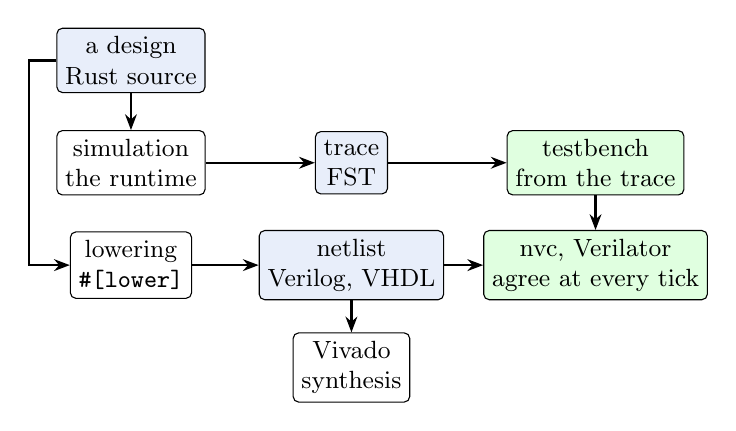
\begin{tikzpicture}[x=1cm, y=1cm]
  \node[art] (src) at (0,1.3) {a design\\Rust source};
  \node[box] (sim) at (0,0) {simulation\\the runtime};
  \node[art] (fst) at (2.8,0) {trace\\FST};
  \node[chk] (tb) at (5.9,0) {testbench\\from the trace};
  \node[box] (low) at (0,-1.3) {lowering\\\code{\#[lower]}};
  \node[art] (net) at (2.8,-1.3) {netlist\\Verilog, VHDL};
  \node[chk] (nvc) at (5.9,-1.3) {nvc, Verilator\\agree at every tick};
  \node[box] (syn) at (2.8,-2.6) {Vivado\\synthesis};
  \draw[flow] (src) -- (sim);
  \draw[flow] (src.west) -- ++(-0.35,0) |- (low.west);
  \draw[flow] (sim) -- (fst);
  \draw[flow] (fst) -- (tb);
  \draw[flow] (tb) -- (nvc);
  \draw[flow] (low) -- (net);
  \draw[flow] (net) -- (nvc);
  \draw[flow] (net) -- (syn);
\end{tikzpicture}
\caption{One source, three forms. The runtime simulates it and writes a
trace; the lowering emits its netlist; a testbench generated from the
trace replays it into the netlist under nvc and Verilator, and the
build fails unless every register and output agrees at every tick.}
\label{fig:p-system}
\end{figure}

The paper presents the system in that order. Section~\ref{sec:p-lang}
is the language: what a unit is, how time is modelled, how units are
wired, and how control flow on a signal is spelled.
Section~\ref{sec:p-sim} is the simulation and its traces.
Section~\ref{sec:p-lower} is the lowering and the checks that close
the loop. Section~\ref{sec:p-vreteno} is Vreteno, an RV32IM core
written in the language, from a reference model to synthesis.
Section~\ref{sec:p-results} gathers the numbers.

\section{The Language}
\label{sec:p-lang}

\subsection{A unit}

Listing~\ref{lst:p-counter} is a complete unit: a counter that ticks
an output once every eight cycles while enabled. It is the unit on
the project's cheat sheet, and it shows everything a unit has. The
struct holds the state, one register of three bits. The
\code{Unit<In, Out>} trait names the ports as type parameters, which
\code{\#[lower]} fills in from \code{run}, whose arguments they are:
an input wire and an output wire here, channels or tuples of either
elsewhere. The body is one
\code{loop}. Its first statement waits for the rising edge of the
default clock; then it reads, plainly, the register and the input;
then it drives, with \code{with!} the register under its condition
and with \code{set} an output wire. The attribute \code{\#[lower]} says
the unit lowers, Section~\ref{sec:p-lower}, and \code{derive(Trace)}
names its fields in a waveform.

\lstinputlisting[rangebeginprefix=//\ begin\{,rangebeginsuffix=\},rangeendprefix=//\ end\{,rangeendsuffix=\},includerangemarker=false,linerange=unit-unit,caption={A unit: state, ports, one loop that waits, reads and drives. From \code{ex\_cheat.rs}.},label={lst:p-counter}]{lib/examples/ex_cheat.rs}

Values are \code{Bit}, IEEE 1164's nine-valued \code{Logic}, and the
sized vectors \code{U<N>} and \code{I<N>}, with Rust's operators for
arithmetic, shifts, bitwise logic and the compares, and methods for
what has no operator: \code{slice}, \code{concat}, \code{sext},
\code{zext}, the arithmetic shift and the signed compare. A struct of values with \code{derive(Value)} is a value with
a width, and a transaction that moves over a channel is such a struct
with \code{derive(Transaction)}. There is no width arithmetic in the
type system, since stable Rust has none; a width that is the sum of
two others is stated, as \code{concat::<\_, M>} states it, the
operand's width left to Rust.

\subsection{Time}

Time runs in ticks. A clock is a type with a period and a phase in
ticks, and its rising edge is an event a process waits for. The
executor polls every process once per tick and then commits the
drives; a process that has crossed an edge at this tick cannot cross
it again, so a second wait written after a first waits for the next
edge. Fig.~\ref{fig:p-time} draws the rule. A process waits, then
reads: a register, in an expression or through \code{get}, is what
the last edge latched, a wire's \code{get} what it carries, a
memory's \code{read} its
asynchronous port. Drives are deferred: \code{set} takes effect at the
end of the tick, so a read after a drive in the same iteration still
sees what the edge latched, as it does in hardware. The default clock
has period two, so its falling edge is a tick of its own and can be
waited for as well.

\begin{figure}[htbp]
\centering
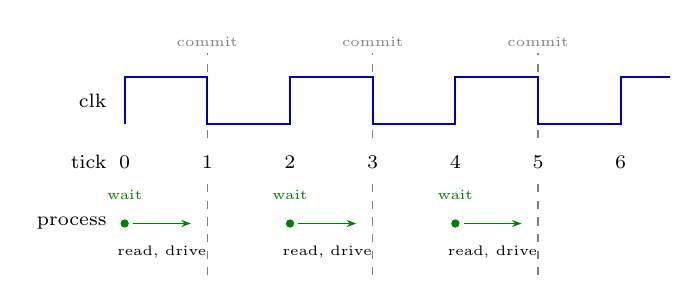
\begin{tikzpicture}[x=1.05cm, y=0.6cm]
  \foreach \t in {0,2,4} {
    \draw[dashed, gray] (\t+1,2.7) -- (\t+1,4.5);
    \draw[dashed, gray] (\t+1,-0.2) -- (\t+1,1.8);
    \node[font=\tiny, gray] at (\t+1,4.75) {commit};
  }
  \draw[thick, blue!70!black] (0,3) -- (0,4) -- (1,4) -- (1,3) -- (2,3) -- (2,4) -- (3,4) -- (3,3) -- (4,3) -- (4,4) -- (5,4) -- (5,3) -- (6,3) -- (6,4) -- (6.6,4);
  \node[left, font=\scriptsize] at (-0.1,3.5) {clk};
  \foreach \t in {0,...,6} { \node[font=\scriptsize] at (\t,2.2) {\t}; }
  \node[font=\scriptsize, left] at (-0.1,2.2) {tick};
  \node[left, font=\scriptsize] at (-0.1,0.9) {process};
  \foreach \t in {0,2,4} {
    \fill[green!50!black] (\t,0.9) circle (1.5pt);
    \node[font=\tiny, green!50!black] at (\t,1.5) {wait};
    \draw[-{Stealth[length=1.2mm]}, green!50!black] (\t+0.1,0.9) -- (\t+0.8,0.9);
    \node[font=\tiny] at (\t+0.45,0.3) {read, drive};
  }
\end{tikzpicture}
\caption{The model of time. A process waits for an edge, reads state
as that edge left it, and drives; the drives commit at the end of the
tick. One wait per edge: the next wait is the next edge.}
\label{fig:p-time}
\end{figure}

\subsection{Wires and channels}

A wire is created once and split into two ends, \code{Out} and
\code{In}; \code{Out} is not \code{Clone}, so a second driver is a
value that cannot be made, and the oldest error in hardware design
arrives as a move error. A channel is a transaction plus the
handshake the language supplies, split into \code{Tx} and \code{Rx}.
Its runtime form is an elastic buffer of two, Fig.~\ref{fig:p-chan}:
a send is an offer, \code{valid} and \code{data} this tick and the
transaction in the buffer at the end of it, allowed when there is
room; a receive is a take, \code{ready} this tick and the head gone
at the end of it. Both commit as register drives do, so two units
that run every cycle pass one transaction per cycle with
\code{valid} and \code{ready} registered on both sides, and no
combinational path joins them. A receiver's \code{wait} is an event
like an edge: the next edge at which the channel holds a transaction.

\begin{figure}[htbp]
\centering
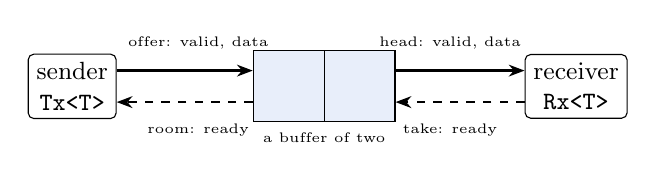
\begin{tikzpicture}[x=1cm, y=1cm]
  \node[box] (tx) at (0,0) {sender\\\code{Tx<T>}};
  \node[draw, fill=tint, minimum width=18mm, minimum height=9mm] (buf) at (3.2,0) {};
  \draw (buf.north) -- (buf.south);
  \node[font=\tiny] at (3.2,-0.65) {a buffer of two};
  \node[box] (rx) at (6.4,0) {receiver\\\code{Rx<T>}};
  \draw[flow] ([yshift=2mm]tx.east) -- ([yshift=2mm]buf.west);
  \node[font=\tiny] at (1.6,0.55) {offer: valid, data};
  \draw[flow, dashed] ([yshift=-2mm]buf.west) -- ([yshift=-2mm]tx.east);
  \node[font=\tiny] at (1.6,-0.55) {room: ready};
  \draw[flow] ([yshift=2mm]buf.east) -- ([yshift=2mm]rx.west);
  \node[font=\tiny] at (4.8,0.55) {head: valid, data};
  \draw[flow, dashed] ([yshift=-2mm]rx.west) -- ([yshift=-2mm]buf.east);
  \node[font=\tiny] at (4.8,-0.55) {take: ready};
\end{tikzpicture}
\caption{A channel. The sender offers into a two-entry buffer and reads
whether there is room; the receiver takes from its head. Every wire is
registered at the buffer, so neither side sees the other's logic.}
\label{fig:p-chan}
\end{figure}

A clock-domain crossing is a type, \code{Crossing<T, A, B>}, and the
only way a value in clock \code{A} becomes one in clock \code{B}; a
wire whose ends are in different clocks does not type-check. An
interface is declared once with its members and its roles, and
\code{interface!} emits a struct per role with the directions the
role has, so a bus master, a target and a monitor are three views of
one declaration.

\subsection{Control flow on a signal}

Hardware does not branch: both arms of a choice exist and a
condition selects. Three macros spell that, each named for what it
is rather than for the Rust it resembles, and Rust's \code{if} is
read the same way. \code{with!(self <= \{ c ? r: v \})} is the drives
of the unit, each under its condition, a group of them under one
with an \code{else}, and \code{when!(c => self \{ r: v \})} the group
with the condition first: both arms exist, a multiplexer chooses,
nothing branches. \code{case!} is the group with many arms, Rust
patterns with
guards and alternatives, the first match winning, so a state machine
is one \code{case!} over its state register. An \code{if} over a
\code{bool}, with the drives under it written as \code{set}, and
its \code{else if} and \code{else}, is the same priority chain, and
its arms nest. \code{select!} chooses among values rather than
drives, \code{match} on a value by another name, and lowers to a
chain of multiplexers; \code{mux} is its two-arm case. Listing~\ref{lst:p-alu} is the Vreteno core's ALU, a
\code{select!} over the function code, in a function under
\code{\#[lower]}, which the lowering writes in where the step calls
it.

\lstinputlisting[rangebeginprefix=//\ begin\{,rangebeginsuffix=\},rangeendprefix=//\ end\{,rangeendsuffix=\},includerangemarker=false,linerange=alu-alu,float,caption={\code{select!}: the ALU of the Vreteno core, one value chosen by the function code. From \code{core.rs}.},label={lst:p-alu}]{cpu/vreteno/src/core.rs}

\subsection{Pipelines and configurations}

An \code{async fn} of awaited operators is a pipeline: each operator
takes the cycles its implementation takes, a value alive across an
await is a register, and the depth follows from the operators rather
than from the source. \code{\#[pipeline(mul = 3, add = 1)]} emits the
Verilog of such a function with the stated latencies, and the same
function with \code{mul = 1} is two stages shorter without an edit. A
configuration is a trait with associated types and constants, a
build is a type alias, and a design is generic over its
configuration; \code{main} names the build, and elaboration is the
program running.

\section{Simulation and Traces}
\label{sec:p-sim}

\code{Running::new(unit.run(inputs, outputs))} is a design under
test, stepped a tick or a cycle at a time while the testbench reads
its wires between steps; \code{Reg} and \code{Mem} give out second
handles for that. \code{Wave::from\_env} names what to watch, by the
field names \code{derive(Trace)} registered, and writes an FST or a
VCD where the environment points; a compound value is one vector and
one signal per field beside it, and an enum is written with its
variant names. Fig.~\ref{fig:p-counter} is the counter of
Listing~\ref{lst:p-counter}, drawn by the build from the trace the
run wrote, through the project's converters and a TikZ generator; no
figure in this paper was drawn by hand.

\begin{figure}[htbp]
\centering
\input{paper_cheat_timing.tex}
\caption{The counter, from its trace: \code{enable} drops at cycle 10,
\code{n} counts while it is high, \code{tick} marks seven.}
\label{fig:p-counter}
\end{figure}

\section{From Source to Netlist}
\label{sec:p-lower}

\subsection{The lowering}

\code{\#[lower]} reads a unit's \code{run} as it is written and
builds a netlist from it, without a second language: one loop, or
several under \code{join2}, each a process on the rising or the
falling edge of its clock and a clocked block of its own; register
and port reads into names, \code{with!}, \code{when!},
\code{case!} and \code{select!}, the datapath operators, memories
written through \code{at} and read by index, and channel ports as a
valid/ready handshake whose wait guards the drives. A \code{let} that
computes is a wire named for it, so the netlist reads as the source
does. What the macro does not read it refuses with a message that
names the construct, and the subset it reads is also plain Rust: a
unit that lowers is the unit that simulates, one file. A unit whose
fields are units lowers too: its \code{run} makes the channels
between the children and joins their \code{run}s, and the netlist
is one module holding an instance of each child's, every channel
between them the runtime's buffer of two as a module of its own, so
a design composed of parts is checked whole at its ports.
Listing~\ref{lst:p-netlist} is what the counter became.

\lstinputlisting[style=ascii,caption={The counter's Verilog, as the build printed it. The VHDL says the same.},label={lst:p-netlist}]{out_cheat.txt}

\subsection{The checks}

A netlist that is only printed is a claim. The build simulates it,
twice. The example is run with two environment variables set, so
beside its trace it writes the unit's VHDL and Verilog; a generator
reads the trace and the unit's ports and writes a testbench, in VHDL
and again in Verilog, that replays the trace's inputs into the entity
and asserts, tick by tick, that its registers and outputs are what
the trace holds; nvc simulates the VHDL and Verilator the Verilog,
both built from source by the build; and each test passes only if
every comparison held. The testbench's timing is the model of time
made literal: an input the trace holds at tick $2k$ is applied at
$2k-1$, a register is checked at $2k+1$, a wire at $2k-1$, and a
channel's registered inputs a tick later than a wire's.
Table~\ref{tab:p-checked} lists the units that pass;
Fig.~\ref{fig:p-stage} is one of them, a stage between two channels,
whose handshake on both sides is what its testbench replays. A unit
is also checked live: a Verilog or VHDL module becomes a unit of the
runtime, Verilator in process or nvc as a child process behind it,
and the examples document runs the stage beside its own Verilog and
its own VHDL in three pipelines on the same offers, which take the
same words at the same ticks.

\begin{table}[htbp]
\caption{Lowered units simulated against their traces.}
\label{tab:p-checked}
\centering
\begin{tabular}{@{}lll@{}}
\toprule
Unit & What it shows & Under \\
\midrule
counter & a register, \code{with!}, an output & nvc, Verilator \\
sampler & two processes, one per edge & nvc, Verilator \\
blinky & a configuration's constants baked in & nvc, Verilator \\
sequencer & \code{case!} on a state enum, guards & nvc, Verilator \\
ALU & ten operators by \code{case!} & nvc, Verilator \\
scratchpad & a memory written and read & nvc, Verilator \\
decoder & \code{slice}, \code{concat}, \code{sext}, \code{select!} & nvc, Verilator \\
stage & two channels, the handshake & nvc, Verilator \\
MAC & \code{mul::<M>}, a product at a stated width & nvc, Verilator \\
tap & a send under \code{if}, a receive with no wait & nvc, Verilator \\
buffer & the channel as hardware, against the runtime's & nvc, Verilator \\
divider & internal wires kept as fields, seen and checked & nvc, Verilator \\
Gray counter & functions under \code{\#[lower]}, inlined & nvc, Verilator \\
Vreteno & the whole core, 732 ticks & nvc, Verilator \\
router & the bus fanned out by address, the same run & nvc, Verilator \\
data memory & a device on the core's bus, the same run & nvc, Verilator \\
timer & a device on the core's bus, the same run & nvc, Verilator \\
serial port & a device on the core's bus, the same run & nvc, Verilator \\
FIFO & \code{D} words between two channels & nvc, Verilator \\
station & two tagged inputs, beside hand Verilog & nvc, Verilator \\
stream ALU & four latencies, results out of order & nvc, Verilator \\
top & a unit of units, a station feeding the ALU & nvc, Verilator \\
\bottomrule
\end{tabular}
\end{table}

\begin{figure}[htbp]
\centering
\input{paper_stage_timing.tex}
\caption{A stage between two channels, from its trace: a word offered
every other cycle is taken, passed on incremented in the same cycle,
and counted. The netlist agrees at every tick.}
\label{fig:p-stage}
\end{figure}

The second simulator earned its place on its first run. Every unit's
VHDL had agreed with its trace; the same units' Verilog, from the
same statements, had two defects VHDL cannot have, an unsized number
inside a concatenation and a shift made logical by Verilog's
whole-expression signedness, and neither showed until the Verilog was
simulated. Both were found by the core and fixed in the emitter.

\section{Vreteno}
\label{sec:p-vreteno}

Vreteno is a 32-bit RISC-V core, the RV32I base integer set with the
M extension, and the largest design in the language. Fig.~\ref{fig:p-core} is its
structure. It is one unit and one process. The fetch stage reads the
instruction memory at the program counter into an instruction
register, with its program counter and a valid bit. The execute stage
decodes the fields of the word in that register with \code{slice},
\code{concat} and \code{sext}, reads two operands from the register
file, computes with the ALU of Listing~\ref{lst:p-alu}, sends a
store or a load out on the bus, where the data memory is a device
like the timer and the serial port and a load's answer comes back
into the writeback registers, and, on a taken branch or a jump,
redirects the fetch
and squashes the word fetched that cycle, which is the one-cycle
penalty. The writeback stage extends a loaded word, writes the
register file and retires; an operand the writeback stage is about
to write is forwarded into execute, except a loaded one, which lands
at the edge and would be too late: the instruction that wants it
waits one cycle, the only stall there is. The core
has machine-mode traps: an \code{ecall} or a word it does not know
saves its address and cause in \code{mepc} and \code{mcause},
saves and clears the interrupt enable in \code{mstatus}, and
redirects to \code{mtvec} as a taken branch redirects; \code{mret}
returns; an interrupt line, pending in \code{mip} and enabled in
\code{mie}, is taken in place of the instruction in execute, which
retires writing nothing; a bus of two channels, a request out and
the word read back, through a router that decodes a device per
address range, on which a timer of sixty lines raises the second
interrupt when its count reaches its compare, a serial port says what the program writes and takes what
a terminal types, and the data memory itself is a device, the
channels between them all being the runtime's buffer of two as
hardware; the six CSR instructions read and write the
eight control registers. Multiply and divide are one sequencer over
the
magnitudes, a multiply one step in the part's DSP blocks and a
division thirty-two restoring steps, the signs put back at the end,
and the instruction stalls for them, off the critical path. The whole is written in the subset the
lowering reads,
Listing~\ref{lst:p-fetch} being the fetch's drives, so the one file
simulates and is a netlist.

\begin{figure}[htbp]
\centering
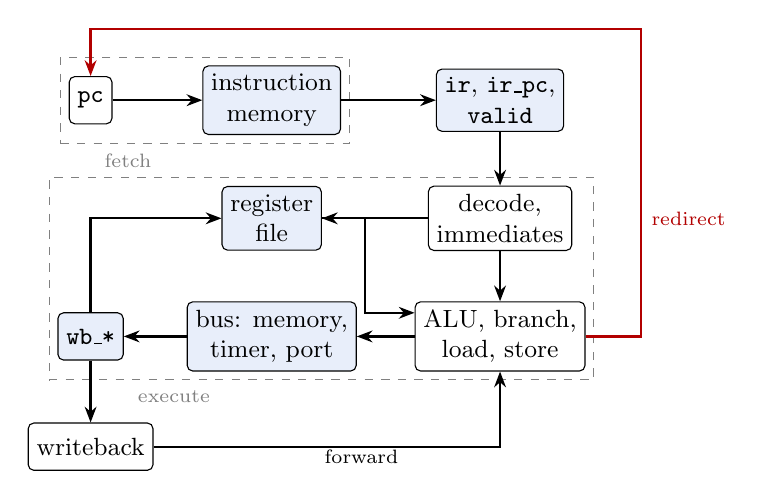
\begin{tikzpicture}[x=1cm, y=1cm]
  \node[box] (pc) at (0,0) {\code{pc}};
  \node[art] (imem) at (2.3,0) {instruction\\memory};
  \node[box, fill=tint] (ir) at (5.2,0) {\code{ir}, \code{ir\_pc},\\\code{valid}};
  \node[box] (dec) at (5.2,-1.5) {decode,\\immediates};
  \node[art] (regs) at (2.3,-1.5) {register\\file};
  \node[box] (alu) at (5.2,-3) {ALU, branch,\\load, store};
  \node[art] (dmem) at (2.3,-3) {bus: memory,\\timer, port};
  \node[box, fill=tint] (wbr) at (0,-3) {\code{wb\_*}};
  \node[box] (wb) at (0,-4.4) {writeback};
  \draw[flow] (pc) -- (imem);
  \draw[flow] (imem) -- (ir);
  \draw[flow] (ir) -- (dec);
  \draw[flow] (dec) -- (regs);
  \draw[flow] (regs.east) -- ++(0.55,0) |- ([yshift=3mm]alu.west);
  \draw[flow] (dec) -- (alu);
  \draw[flow] (alu) -- (dmem);
  \draw[flow] (dmem) -- (wbr);
  \draw[flow] (wbr) -- (wb);
  \draw[flow] (wb.east) -| node[lbl, pos=0.3, below] {forward} (alu.south);
  \draw[flow] (wbr.north) -- (wbr.north |- regs.west) -- (regs.west);
  \draw[flow, red!70!black] (alu.east) -- ++(0.7,0) |- ([yshift=6mm]pc.north) -- (pc.north);
  \node[font=\scriptsize, text=red!70!black, anchor=west] at (7.0,-1.5) {redirect};
  \begin{scope}[on background layer]
    \node[draw, dashed, gray, fit=(pc)(imem), inner sep=3pt, label={[gray, font=\scriptsize]below left:fetch}] {};
    \node[draw, dashed, gray, fit=(dec)(regs)(alu)(dmem)(wbr), inner sep=3pt, label={[gray, font=\scriptsize]below left:execute}] {};
  \end{scope}
\end{tikzpicture}
\caption{Vreteno: three stages in one process. The instruction
register and the writeback registers are the boundaries; a taken
branch, jump or trap redirects the fetch and costs one bubble; the
value in writeback is forwarded into execute, a loaded one by a
stall of one cycle instead.}
\label{fig:p-core}
\end{figure}

\lstinputlisting[rangebeginprefix=//\ begin\{,rangebeginsuffix=\},rangeendprefix=//\ end\{,rangeendsuffix=\},includerangemarker=false,linerange=fetch-fetch,float,caption={The fetch's drives: the next counter as two candidates, the early conditions folded into each and the late redirect choosing between them; the instruction register under a \code{case!}. From \code{core.rs}.},label={lst:p-fetch}]{cpu/vreteno/src/core.rs}

The core is checked three ways. A reference model of the instruction
set, written as a plain program over the architectural state, runs in
lockstep with it: the model steps when the core retires an
instruction, and after every cycle the program counter, the
thirty-one registers, the control registers and the halt must agree,
and at the halt the data memory must. The demonstration program,
which traps twice, and sixty-four random programs of two hundred
instructions, with traps among them, pass; a broken shift, a branch
that does not squash, or a return from a trap with the wrong status
fails at its first use. The netlist is
checked as every lowered unit is, under nvc and Verilator, with the
program in its instruction memory. And the Verilog is synthesized,
Table~\ref{tab:p-synth}, on an Artix-7 with a clock constraint of ten
nanoseconds, by Vivado, which the build installs itself from the
vendor's archive into a cache the machine shares. The instruction
memory became a read-only memory in one block RAM tile, the data
memory's four byte lanes four block RAMs in two, since the third
stage registers their read, and the register file distributed RAM.
Placed and routed with the same constraint, the core meets ten
nanoseconds with 0.315~ns to spare; the critical path runs from the
writeback's destination register through the forwarding compare
into an operand and the jump's add to the instruction memory's
address, a jump through a register the instruction before is still
writing, and is three quarters routing. Fig.~\ref{fig:p-vreteno} is the opening of the
demonstration, from the trace, and Fig.~\ref{fig:p-uart} the serial
port's line as the demonstration's O goes out, from the same trace:
the write into the port, then the start bit, the byte low bit first
and the stop bit, four cycles each.

\begin{table}[htbp]
\caption{Vreteno on an Artix-7, after synthesis.}
\label{tab:p-synth}
\centering
\begin{tabular}{@{}lr@{}}
\toprule
Resource & Used \\
\midrule
LUTs, as logic & 1952 \\
LUTs, as distributed RAM & 48 \\
Flip-flops & 486 \\
Block RAM tiles & 1 \\
DSP blocks & 4 \\
Errors, critical warnings & 0 \\
\bottomrule
\end{tabular}
\end{table}

\begin{figure}[htbp]
\centering
\input{paper_vreteno_out_timing.tex}
\caption{A byte out on Vreteno's serial port, from the trace: the
write reaches the port and the line carries the frame, a start bit,
the byte low bit first and a stop bit, four cycles each; the later
requests are the program's polls for the next byte.}
\label{fig:p-uart}
\end{figure}

\begin{figure}[htbp]
\centering
\input{paper_vreteno_timing.tex}
\caption{Vreteno's first cycles, from its trace: reset, then an
instruction per edge with the fetch counter running ahead, and the
writeback decoded into its register and value.}
\label{fig:p-vreteno}
\end{figure}

\section{Results}
\label{sec:p-results}

What the system does, in numbers from the build that produced this
paper. The runtime is five Rust modules, one macro crate and one
crate of parts, with one
external crate, an FST writer. Thirty examples compile, each one
concept, and every one that runs writes a waveform the examples
document draws. Eighteen lowered units, Table~\ref{tab:p-checked}, are
simulated as VHDL under nvc and as Verilog under Verilator against
the traces their Rust simulations wrote, and agree at every tick;
forty-one tests run under \code{bazel test //...}, and every one of them
is hermetic, the simulators built from source and the synthesis tool
installed by the build. Vreteno is 815 lines of core, 78 of data
memory, 98 of timer,
62 of router and 89 of serial port, checked in lockstep against a
364-line model on a demonstration program and sixty-four random
ones, with interrupts raised at random, checked as a netlist on 732
ticks with every register compared at each, synthesized in two
minutes to the figures of Table~\ref{tab:p-synth}, placed and
routed at 100~MHz, and programmed into the board, where it said OK on
its serial port and echoed the three bytes typed back, the six bytes
its simulation had produced, and lit its LEDs as the board top says,
which an author saw and photographed: the language is proven on
hardware, end to end, from a Rust source to a board that answers. Twelve documents
describe the system, this one
included, and each is built by the same command that builds the
designs, with every listing included from the tree and every figure
drawn from a trace, so none can drift from the code.

\section{Related Systems}
\label{sec:p-related}

Chisel~\cite{bachrach2012} and SpinalHDL embed a hardware language in
Scala with the same structural architecture: a module is a class, a
bundle has directions, \code{when} and \code{Mux} are control flow on
a signal, and elaboration is the program running. TxHDL's structural
half is that architecture in Rust, where a second driver is a move
error and a configuration is a type. Its behavioural half, an
\code{async fn} that is a sequence, a pipeline or a process according
to how it is driven, has no counterpart in Chisel; its nearest
relatives are XLS~\cite{xls}, whose Rust-shaped DSLX the compiler
schedules into pipelines, and Calyx~\cite{calyx}, whose \code{seq}
and \code{par} are an \code{await} and a \code{parallel!} seen from
the other side. RHDL~\cite{rhdl} embeds a hardware language in Rust
with the clock domain as a type parameter, which TxHDL takes
directly. What sets TxHDL apart from all of them is not any one
construct but the loop the build closes: one source, three forms,
and a test that fails when they disagree.

\section{Where the Work Is}
\label{sec:p-where}

The work is done on the authors' own Forgejo instance,
\code{git.hdlfactory.com}, in the repository \code{HDL/txhdl}: the
mainline, the pull requests, the continuous build that renders every
document and runs every check, and the nightly release of every
document as a PDF. That instance is by invitation. A mirror of the
mainline is public on GitHub, at \code{github.com/filmil/hdl-txhdl},
pushed on every change and never forced; it holds the same tree, the
same history and the same releases, and is read-only. So the tree
this paper is built from is public, and every listing in it can be
read there; the way in for a contributor is the corresponding author,
who opens an account on the instance. The whole of it is under the
Apache License, version 2.0.

\section{Conclusion}
\label{sec:p-conclusion}

A hardware description language can be a Rust library. The language
is small enough to fit on one page, the runtime simulates it with a
stated model of time, the lowering turns it into Verilog and VHDL,
and the build holds the three to one behaviour under two simulators.
A RISC-V core written in it runs, lowers, is checked against its own
trace, runs at 100~MHz on an Artix-7 with its data memory in block
RAM, and has run on the board, saying on its serial port what its
simulation said: the language is proven on hardware. The path that
limits the clock is a jump through a register.

\begin{thebibliography}{10}

\bibitem{cover}
F.~Filmar and D.~Janković, ``TxHDL documents,'' project repository
\code{HDL/txhdl}, \code{//docs:cover}, 2026.

\bibitem{bachrach2012}
J.~Bachrach et al., ``Chisel: Constructing hardware in a Scala embedded
language,'' in \emph{Proc. 49th Design Automation Conference}, 2012.

\bibitem{xls}
Google, ``XLS: Accelerated HW synthesis,'' \code{github.com/google/xls}.

\bibitem{calyx}
R.~Nigam et al., ``A compiler infrastructure for accelerator
generators,'' in \emph{Proc. ASPLOS}, 2021.

\bibitem{rhdl}
S.~Roantree, ``RHDL: A hardware description language embedded in Rust,''
\code{github.com/samitbasu/rhdl}.

\end{thebibliography}

\end{document}
